%! TEX root = ../main.tex
We previously examined the correction proposed by \citet{vermeulen2018} for differential unit non-response (Section~\ref{sec:measuring-wealth}). The intuition is that household surveys fail to capture billionaires at the extreme right tail. Since this group is small and largely identifiable, observing its wealth allows us to recover the extended Pareto tail. While effective, the method is sensitive to the threshold chosen to define and estimate the tail (see Section~\ref{sec:results}).

In this section, we discuss an alternative data-driven approach proposed by \citet{blanchet2022weight} that does not rely on a parametric Pareto assumption. Due to the lack of tabulated wealth tax data for Chile, we do not apply this correction to wealth inequality but illustrate it for income inequality using the National Socioeconomic Characterization Survey (CASEN) waves 2017 and 2022 \citep{casen2017, casen2022}.

\subsection*{The Blanchet-Flores-Morgan (BFM) Technique}\label{sec:bfm}
\citet{blanchet2022weight} develop a calibration-based method to reconcile survey microdata with tabulated tax data. Unlike \citet{vermeulen2018}, the method does not assume a Pareto tail from an ad hoc cutoff $w_{\min}$. Instead, it endogenously determines a \textit{merging point} $y^{*}$ above which tax data become more reliable than the survey, and then corrects the survey via reweighting and imputation while preserving its demographic structure.

\paragraph{The Merging point}\label{sec:bfm-merging}
Let $f(y)$ and $F(y)$ denote the income density and cumulative distribution, with subscripts $s$ for survey and $t$ for tax tabulations. Define the density ratio and the cumulative ratio as:
\begin{equation}
    \theta(y) = \frac{f_{s}(y)}{f_{t}(y)}, \qquad \Theta(y) = \frac{1-F_{s}(y)}{1-F_{t}(y)}.
    \label{eq:theta-Theta}
\end{equation}
If the survey were representative at income $y$, $\theta(y)=\Theta(y)$. The central assumption in \citet{blanchet2022weight} is that representativeness is constant up to $y^{*}$ and strictly decreasing thereafter, reflecting systematic under-coverage of the rich due to non-response and misreporting. The merging point $y^{*}$ is then defined as the largest income such that the density ratio and the cumulative ratio coincide:
\begin{equation}
    y^{*} = \sup \{ y : \theta(y) = \Theta(y) \}.
    \label{eq:merging-point}
\end{equation}
Below $y^{*}$ the survey is trusted; above $y^{*}$ the tax data dominate. By construction, $y^{*}$ is higher (more conservative) than the quantile-crossing point used in earlier hybrid methods, thereby minimizing unnecessary distortion of the survey \citep[see Appendix~A.3 in][]{blanchet2022weight}. Crucially, to guarantee that such an empirical intersection exists and is analytically unique—both in continuous distributions and across discrete quantile brackets—formal mathematical proofs are provided in Appendix~\ref{app:merging-point-proof}.

\paragraph{Estimation of $y^{*}$.}
The practical problem is to locate $y^{*}$ from tabulated tax data and survey microdata without imposing an arbitrary threshold. We construct a fractal percentile grid with 126 bins: 99 bins of 1~pp covering $0$--$99\%$, followed by $9$ bins of $0.1$~pp for $99$--$99.9\%$, $9$ bins of $0.01$~pp for $99.9$--$99.99\%$, and $9$ bins of $0.001$~pp for $99.99$--$99.999\%$, as shown in Figure~\ref{fig:fractal}. The SII tabulations are interpolated via generalized Pareto interpolation \citep{blanchet2022generalized}\footnote{Implemented in \texttt{source/bfm.py:61-116} (\texttt{interpolate\_tax\_tabulation}), which shells out to R through \texttt{source/gpinter\_bridge.R}; without R and the \texttt{gpinter} package the code falls back to linear interpolation with a warning.} using, for each bracket, the number of taxpayers and mean income. The first SII bracket is exempt ($0$--$13.5$~UTA), so the fiscal CDF is adjusted and evaluated only above the second bracket lower bound $y_2$:
\begin{equation}
F_t(y_2) = 1 - \kappa + \kappa w_1,
\label{eq:ft-y2}
\end{equation}
where $\kappa$ is taxpayers over adult population (fiscal coverage) and $w_1$ is the first-bracket share in the raw SII tabulation. The grid therefore runs over $[F_t(y_2), 1]$.

Figure~\ref{fig:fractal} shows why the binning is called fractal: at each level the $1\%$ tail left unexplained is re-divided by $10$, so resolution grows exactly where non-response is concentrated.

\begin{figure}[H]
    \centering
    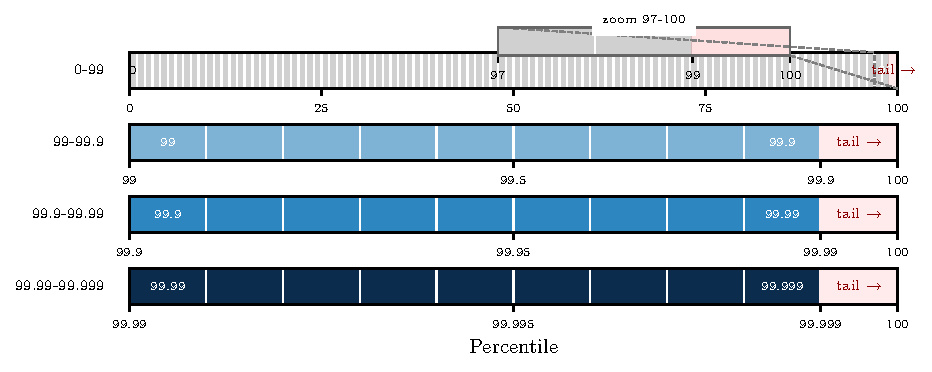
\includegraphics[width=0.85\textwidth]{../../figures/p3/bfm_fractal_bins.pdf}
    \caption{Fractal bins for tax tabulations in \citet{blanchet2022weight}. Each row zooms into the tail (red-hatched) of the row above. The top row covers $0$--$99\%$ with $99$ bins of $1$~pp; subsequent rows split the remaining tail into $9$ bins of $0.1$, $0.01$ and $0.001$~pp, respectively. The inset in the top panel magnifies the $97$--$100\%$ region where the $99\%$ cutoff would otherwise be invisible.}
    \label{fig:fractal}
\end{figure}

Let $d_i$ denote the survey design weight of observation $i$ and $N_s=\sum_{i} d_i$ the survey-weighted population. For bin $k=[y_k,y_{k+1})$ with width $width_k=y_{k+1}-y_k$, let $w_k$ be the tax-data population share of the bin (e.g., $1$~pp, $0.1$~pp) and $\text{share}_{s,k}=\sum_{i: y_i\in bin_k} d_i/N_s$ the corresponding survey share. Histogram densities are $f_{t,k}=w_k/width_k$ and $\tilde{f}_{s,k}=\text{share}_{s,k}/width_k$, so the raw ratio is
\begin{equation*}
\tilde{\theta}_{k}= \frac{\tilde{f}_{s,k}}{f_{t,k}} = \frac{\text{share}_{s,k}}{w_k}= \frac{\sum_{i: y_i \in \text{bin }k} d_i/N_s}{w_k},
\end{equation*}
i.e., the survey share in the bin divided by the tax-data share; $width_k$ cancels but makes explicit that $\tilde{\theta}_k$ compares densities. Because $\tilde{\theta}_{k}$ is noisy, \citet{blanchet2022weight} smooth it via an antitonic (monotonically decreasing) regression:
\begin{equation}
    \min_{\hat{\theta}_{1}\ge \cdots \ge \hat{\theta}_{m}} \sum_{k=1}^{m} w_{k} (\hat{\theta}_{k} - \tilde{\theta}_{k})^{2},
    \label{eq:antitonic}
\end{equation}
where $w_{k}$ is the population share of bin $k$, solved by the Pool Adjacent Violators Algorithm. 

Once $\tilde{\theta}$ is smoothed, the merging point is estimated as the lowest bin $k^{*}$ such that $\hat{\theta}_{k^{*}} < \hat{\Theta}_{k^{*}}$, with fiscal incomes in tabulations interpolated via the generalized Pareto interpolation of \citet{blanchet2022generalized}. $\Theta(y)$ is already stable and can be estimated directly from empirical CDFs:
\begin{equation}
    \hat{\Theta}(y)=\frac{1-\hat{F}_{s}(y)}{1-\hat{F}_{t}(y)}, \quad 
    \hat{F}_{s}(y)=\frac{1}{N_s}\sum_{i=1}^{N_s} d_i\mathbf{1}\{y_i \le y\},
    \label{eq:Theta-hat}
\end{equation}
where $\hat{F}_{t}(y)$ is obtained from the interpolated tax tabulation and $\hat{\Theta}_{k}=\hat{\Theta}(y_k)$ at the lower bound of bin $k$.

\paragraph{Normalization of units.}
Because the SII tabulations count individual taxpayers while CASEN records total household income, the two distributions are not directly comparable. We express both in annual income per adult: each household's income is \texttt{ytotcorh} $\times$ 12 divided by the number of adults aged 20 or older, and the effective weight is the household expansion factor times the number of adults. Without this conversion the household-level survey density cannot be aligned with the individual-level fiscal density.

\paragraph{Reweighting via calibration.}\label{sec:bfm-reweighting}
Given $y^{*}$, the survey is corrected to match tax-data totals above the threshold while preserving representativeness in other dimensions (age, gender, household type). This is achieved through linear calibration \citep{DevilleSarndal1992}, routinely used by statistical agencies. Let $\{(x_{i}, d_{i})\}_{i=1}^{n}$ be the survey sample with $k$-dimensional covariates $x_{i}$ and design weights $d_{i}$, and let $T$ be the vector of known population totals from external sources. Calibrated weights $\{w_{i}\}$ solve:
\begin{equation}
    \min_{\{w_{i}\}} \sum_{i=1}^{n} \frac{(w_{i}-d_{i})^{2}}{d_{i}} \quad \text{s.t.} \quad \sum_{i=1}^{n} w_{i} x_{i} = T, \quad \frac{1}{\alpha} \le \frac{w_{i}}{d_{i}} \le \alpha,
    \label{eq:calibration}
\end{equation}
with truncation $\alpha=5$ to avoid extreme adjustments, followed by a uniform rescaling below and above $y^{*}$ to match exactly the tax-data count above the merging point. Unlike the estimation of $y^{*}$, no shape restriction is imposed on $\theta(y)$ above $y^{*}$; empirical ratios are used directly, including local overestimation due to heaping at round values.

\paragraph{Expanding the support.}
Calibration alone cannot create incomes beyond the survey support $\max(y_{s})$. When tax tabulations extend further, \citet{blanchet2022weight} inflate the sample by splitting each observation $i$ into $k_{i}=[\pi \cdot w_{i}]$ copies with weight $q_{i}=w_{i}/k_{i}$, and assign incomes from the continuous distribution fitted to tax data by generalized Pareto interpolation, preserving the rank of observations. This addresses small-sample bias at the very top, which calibration corrects only asymptotically \citep{DevilleSarndal1992}.

\begin{algorithm}[H]
    \caption{Blanchet-Flores-Morgan (2022) Correction Procedure}\label{alg:bfm}
    \SetAlgoLined
    \KwIn{Survey microdata $\{(y_{i}, d_{i}, x_{i})\}_{i=1}^{N}$; tabulated tax data $\{b_{k}\}_{k=1}^{m}$; calibration totals $T$.}
    \KwOut{Merging point $y^{*}$; calibrated weights $\{w_{i}\}$; augmented sample with corrected shares.}
    \BlankLine
    \tcp{Step 1: Estimate merging point $y^{*}$}
    Interpolate tax tabulations via generalized Pareto; compute $\hat{\Theta}_{k}$ and $\tilde{\theta}_{k}$ per bin; smooth to $\hat{\theta}_{k}$ via antitonic regression \eqref{eq:antitonic}; set $y^{*}$ as first bin with $\hat{\theta}_{k} < \hat{\Theta}_{k}$\;
    \BlankLine
    \tcp{Step 2: Calibration reweighting}
    Solve \eqref{eq:calibration} to obtain $w_{i}$ matching tax-data mass above $y^{*}$ and demographic totals, with truncation $\alpha=5$\;
    \BlankLine
    \tcp{Step 3: Expand support beyond $\max(y_{s})$}
    Duplicate observations as $k_{i}=[\pi w_{i}]$ copies and assign tail incomes from interpolated tax distribution preserving ranks\;
    \BlankLine
    \tcp{Step 4: Recompute inequality indicators}
    Compute corrected top shares and Gini on augmented sample; compare with survey-only baseline\;
\end{algorithm}

Unlike \citet{vermeulen2018}, the BFM procedure is fully data-driven, preserves the joint distribution of income and covariates, guarantees continuity of the density at $y^{*}$, and does not require choosing $w_{\min}$ by visual inspection. Its cost is the need for detailed tabulated tax data covering a sizable share of the population, which is available for income in Chile (SII tabulations) but not for wealth, motivating our application to CASEN income in the next subsection.

\subsection{Data}\label{sec:bfm-data}
We illustrate BFM on income using the National Socioeconomic Characterization Survey (CASEN) for 2017 and 2022 \citep{casen2017, casen2022} and tabulated tax data from the Chilean Internal Revenue Service (SII) \citep[see][for tabulation details]{sii2024personas}. The CASEN microdata are person-level with household identifiers and expansion factors\footnote{See \texttt{source/casen.py:11-28} (\texttt{INCOME\_COLS}, \texttt{load\_casen}) and \texttt{source/casen.py:92-108} (\texttt{to\_household}), plus \texttt{notebooks/05\_data\_exploration.ipynb}; loading uses \texttt{convert\_categoricals=False} to avoid duplicate labels in \texttt{rama4\_sub\_rev3}.}. At the person level $N=216{,}439$ (2017) and $N=202{,}231$ (2022); collapsing to one row per household yields $N_{hh}=70{,}948$ (2017) and $72{,}053$ (2022) with total household income corrected for non-response\footnote{See \texttt{source/casen.py:29-91} (\texttt{income\_overview}, \texttt{summarize\_income}); missingness is $0\%$ for total household income in 2017 and $0.06\%$ in 2022, versus $31$--$44\%$ for uncorrected autonomous income, motivating the choice of total household income; household-level weighted median is CLP~$0.80$M (2017) and $1.11$M (2022).}. We use total household income with survey weights for BFM; per-capita total income is retained for robustness. Household-level data for replication are saved to the processed CASEN household files in \texttt{data/processed}\footnote{See \texttt{notebooks/05\_data\_exploration.ipynb}, Sec.~6 (\texttt{to\_household}, \texttt{OUTPUTDATA}).}. Figure~\ref{fig:casen-income} displays the weighted household income distributions (log scale) and Figure~\ref{fig:casen-lorenz} overlays the corresponding Lorenz curves for 2017 and 2022.
\begin{figure}[H]
    \centering
    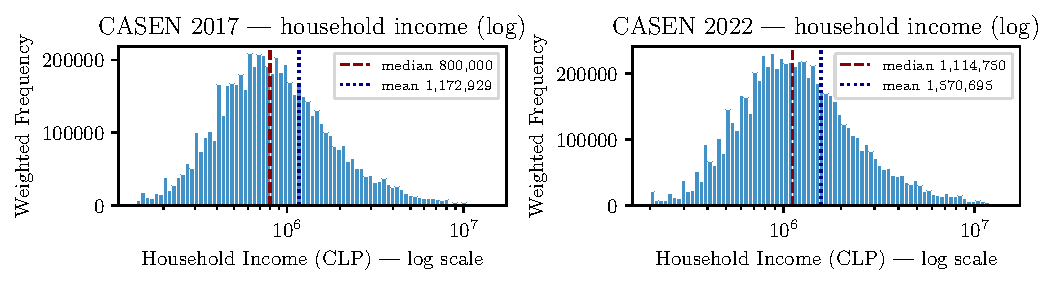
\includegraphics[width=0.85\textwidth]{../../figures/p3/casen_income_dist.pdf}
    \caption{Household income distribution (CASEN, total household income, log scale). Weighted histograms for 2017 and 2022 at household level. Vertical lines mark weighted mean (dotted) and median (dashed). Both years are right-skewed; 2022 shifts right (higher mean/median) but retains a heavy tail. This is the survey density $f_s$ that BFM will compare to $f_t$ from SII tabulations.}
    \label{fig:casen-income}
\end{figure}

\begin{figure}[H]
    \centering
    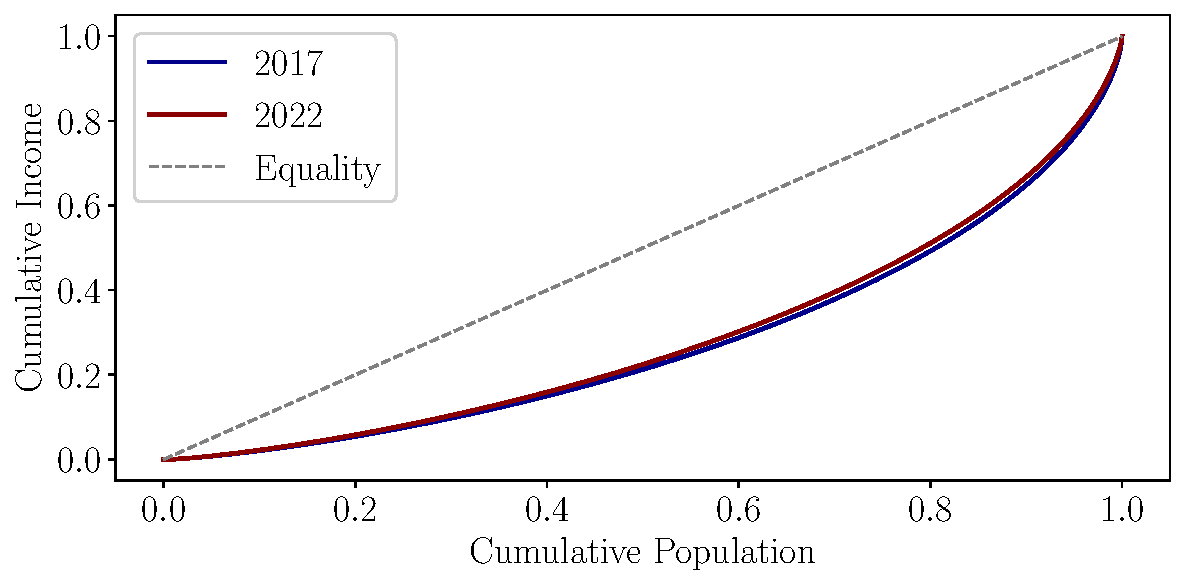
\includegraphics[width=0.60\textwidth]{../../figures/p3/casen_lorenz.pdf}
    \caption{Lorenz curves overlaid (CASEN household income). Cumulative population (weighted) vs.\ cumulative income for 2017 (blue) and 2022 (red), with the $45^{\circ}$ equality line (gray dashed). Proximity of the two curves indicates little change in overall inequality; the gap to the diagonal reflects concentration at the top that motivates the BFM correction.}
    \label{fig:casen-lorenz}
\end{figure}
Tax tabulations are from the SII annual file on natural persons (2005--2024, updated Oct~2025) which reports, by UTA bracket, the number of taxpayers and total income (in MM~CLP) for Global Complementary Tax, Second Category, and Consolidated totals\footnote{See \texttt{source/sii.py:10-118} (\texttt{load\_sii\_pub\_total}, \texttt{sii\_for\_at}) for parsing the double header (rows~6--7) and \texttt{notebooks/05\_data\_exploration.ipynb}, Sec.~5.}. For BFM we use the Consolidated block. The 2020 reform added a top bracket, so the count rises from 7 brackets in 2017 to 8 in 2022, with top brackets \textit{More than 120 UTA (Rate 35\%)} in 2017 and \textit{More than 310 UTA (Rate 40\%)} in 2022; amounts are in MM~CLP at Dec.~31 of each commercial year. Figure~\ref{fig:sii-comparison} compares the Consolidated tabulations by bracket for the two years.
\begin{figure}[H]
    \centering
    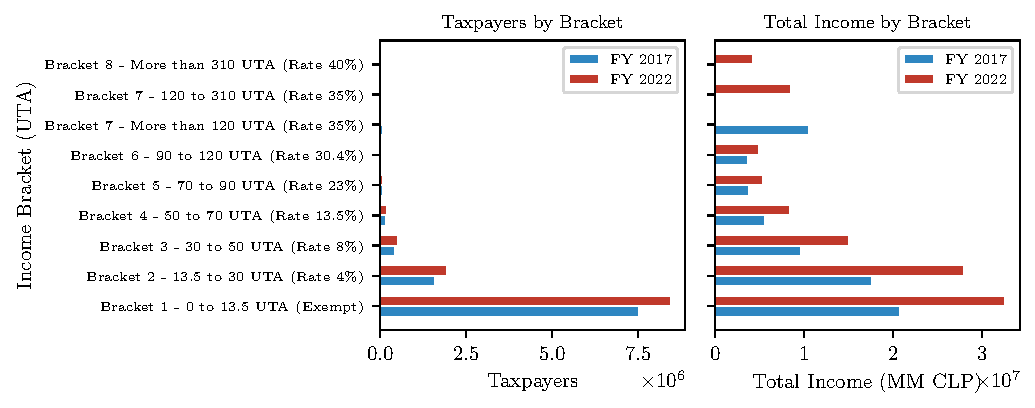
\includegraphics[width=0.95\textwidth]{../../figures/p3/sii_brackets_comparison.pdf}
    \caption{SII tax tabulations (Consolidated) by UTA bracket: 2017 vs.\ 2022 (commercial years, i.e., AT 2018 vs.\ AT 2023). Left: number of taxpayers; right: total income (MM~CLP) per bracket. Bracket labels are translated from Spanish and decimal commas converted to dots; grouping handles the reform-induced change from 7 to 8 brackets (outer join, missing brackets set to 0). This is the fiscal density $f_t$ used to estimate $\tilde{\theta}_k$ and $\hat{\Theta}_k$.}
    \label{fig:sii-comparison}
\end{figure}

\subsection{Results}

Table~\ref{tab:bfm-shares} reports top income shares computed on annual income per adult. The raw CASEN survey understates top incomes relative to the SII tabulations; BFM calibration raises the top-1\% share from 9.17\% to 13.56\% in 2017 and from 7.86\% to 9.40\% in 2022 under the default clip $\alpha=5$. Expanding the support beyond the survey maximum adds a further 0.86~pp in 2017 and 0.36~pp in 2022. In 2022 the required calibration factor exceeds the $\alpha=5$ clip; relaxing it to $\alpha\ge10$ raises the top-1\% share to 10.03\% and, with expansion, to 10.19\%.

\begin{table}[H]
\centering
\caption{Top income shares under BFM correction, annual income per adult (\% of total income)}
\label{tab:bfm-shares}
\small
\begin{tabular}{lcccccc}
\toprule
 & \multicolumn{3}{c}{2017} & \multicolumn{3}{c}{2022} \\
\cmidrule(lr){2-4} \cmidrule(lr){5-7}
Method & Top 10\% & Top 5\% & Top 1\% & Top 10\% & Top 5\% & Top 1\% \\
\midrule
Raw survey & 35.91 & 24.58 & 9.17 & 34.11 & 22.70 & 7.86 \\
BFM calibrated ($\alpha=5$) & 40.16 & 29.27 & 13.56 & 35.43 & 24.12 & 9.40 \\
BFM + support expansion & 40.75 & 29.96 & 14.42 & 35.69 & 24.42 & 9.76 \\
\midrule
2022, $\alpha\ge 10$ & --- & --- & --- & 35.97 & --- & 10.03 \\
2022, $\alpha\ge 10$ + expansion & --- & --- & --- & --- & --- & 10.19 \\
\bottomrule
\end{tabular}
\end{table}

Table~\ref{tab:bfm-params} reports the merging point and calibration diagnostics. Fiscal coverage $\kappa$ is 0.736 in 2017 and 0.763 in 2022. The exempt first bracket shifts the effective start of the fiscal CDF to $F_t(y_2)=0.819$ and 0.804, leaving 45 and 46 bins above $y_2$ in which to search for the merging point. The resulting $y^{*}$ is 68.03~M CLP per year ($\sim$121~UTA) in 2017 and 190.0~M CLP per year ($\sim$271~UTA) in 2022; only 12 survey observations lie above the 2022 threshold.

\begin{table}[H]
\centering
\caption{BFM calibration parameters and merging point}
\label{tab:bfm-params}
\small
\begin{tabular}{lcc}
\toprule
Parameter & 2017 & 2022 \\
\midrule
$y^{*}$ (M CLP/year) & 68.03 ($\sim$121 UTA) & 190.0 ($\sim$271 UTA) \\
$\kappa$ (taxpayer coverage) & 0.736 & 0.763 \\
$F_t(y_2)$ & 0.819 & 0.804 \\
Grid bins used & 45 & 46 \\
Observations above $y^{*}$ & 111 & 12 \\
\bottomrule
\end{tabular}
\end{table}

\begin{figure}[H]
    \centering
    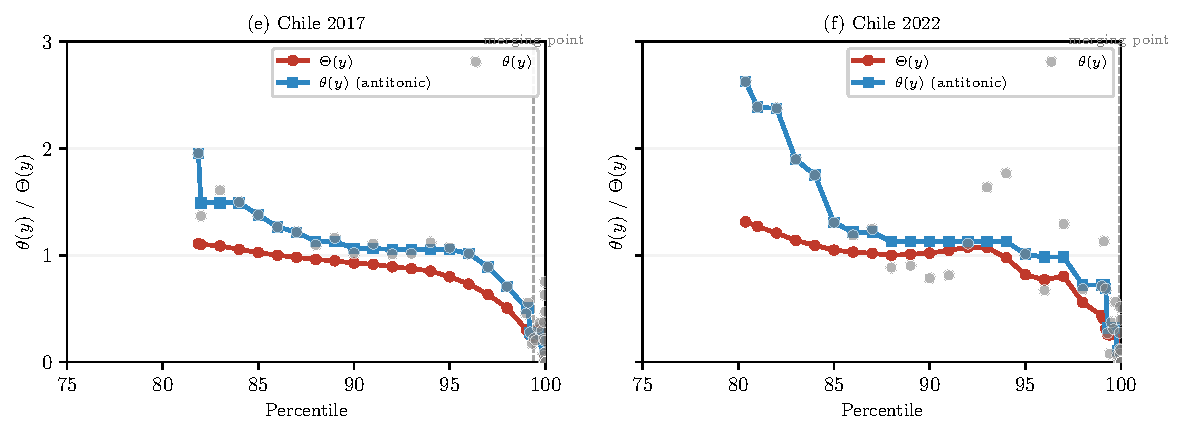
\includegraphics[width=0.95\textwidth]{../../figures/p3/bfm_theta_Theta_real.pdf}
    \caption{BFM empirical diagnostic curves with upper-tail zoom: marginal vs.\ cumulative representativeness ratios for Chile (2017 and 2022). Raw density ratio $\tilde{\theta}(y)$ per fractal bin (gray dots), antitonic isotonic regression $\hat{\theta}(y)$ (blue line with squares), and cumulative ratio $\hat{\Theta}(y)$ (red line with circles). The main axes display the overall trajectory across the upper distribution ($P \ge 75\%$). The inset axes zoom in on the extreme right tail ($P \ge 98\%$), clearly resolving the crossing of $\hat{\theta}(y)$ and $\hat{\Theta}(y)$ at the endogenous merging point $y^*$ (marked by the dashed gray vertical line and labeled percentile). Panel (e) depicts commercial year 2017 ($y^* = 68.03$~M CLP/year, $P99.40$, 111 observations above $y^*$); Panel (f) depicts commercial year 2022 ($y^* = 190.0$~M CLP/year, $P99.90$, 12 observations above $y^*$).}
    \label{fig:bfm-theta-Theta}
\end{figure}

Figure~\ref{fig:bfm-theta-Theta} plots the empirical trajectory of $\tilde{\theta}(y)$, $\hat{\theta}(y)$, and $\hat{\Theta}(y)$ across the upper percentile distribution for 2017 and 2022, directly replicating the diagnostic specification of \citet[][Figure~6e]{blanchet2022weight}. The raw density ratio $\tilde{\theta}(y)$ (gray dots) exhibits substantial sampling dispersion and local heaping around round income values. However, its antitonic PAVA smoothing $\hat{\theta}(y)$ (blue line with squares) displays a strictly non-increasing profile in the upper tail, empirically corroborating the theoretical monotonicity conditions established in Appendix~\ref{app:merging-point-proof}. The cumulative ratio $\hat{\Theta}(y)$ (red line with circles) remains remarkably stable near unity throughout the domain. 

Comparing the two panels highlights significant structural differences across survey waves:
\begin{itemize}
    \item \textbf{Commercial Year 2017 (Panel~e):} The marginal representativeness rate $\hat{\theta}(y)$ tracks the tax density closely across the 82nd to 96th percentiles ($\hat{\theta} \approx 1.0$--$1.2$), indicating high survey fidelity across the upper-middle class. Above the 98th percentile, $\hat{\theta}(y)$ declines sharply and crosses below $\hat{\Theta}(y)$ at $y^* = 68.03$~M CLP/year ($\sim$121~UTA, approximately P99.4). Because 111 survey households lie above this cutoff, the tail calibration is empirically well-supported and stable, and the required calibration factor $(1 - F_t(y^*))/(1 - F_s(y^*)) = 3.78$ falls safely below the $\alpha = 5$ truncation clip.
    \item \textbf{Commercial Year 2022 (Panel~f):} In contrast, $\hat{\theta}(y)$ starts considerably higher in the lower-tax brackets ($\sim 2.6$ near P80), reflecting substantial post-pandemic nominal income growth and high labor informality. It remains elevated ($\hat{\theta} \approx 1.1$) across P86--P94, and crosses $\hat{\Theta}(y)$ only at an extreme threshold of $y^* = 190.0$~M CLP/year ($\sim$271~UTA, P99.8). This high threshold leaves merely 12 survey households above $y^*$, virtually exhausting the survey sample in the extreme tail. As a consequence, the required calibration factor surges to $6.69$, hitting the $\alpha = 5$ truncation constraint (Table~\ref{tab:bfm-sens-factor}) and underscoring the critical necessity of support expansion to avoid downward bias in top wealth/income shares.
\end{itemize}

\paragraph{Sensitivity.}
Table~\ref{tab:bfm-sens-kappa} shows how the top-1\% share and the merging point vary with assumed fiscal coverage $\kappa$. In 2017 the estimated top-1\% share rises monotonically from 10.93\% to 13.56\% as $\kappa$ moves from 0.40 to the estimated 0.736; $y^{*}$ falls from 70.94~M to 66.37~M CLP and then returns to 68.03~M CLP at the estimated $\kappa$. In 2022 the share is flat at 9.40\% for $\kappa\ge0.50$ because the $\alpha=5$ clip is already binding.

\begin{table}[H]
\centering
\caption{Sensitivity to fiscal coverage $\kappa$}
\label{tab:bfm-sens-kappa}
\small
\begin{tabular}{lccccc}
\toprule
$\kappa$ & 0.40 & 0.50 & 0.60 & 0.70 & Estimated \\
\midrule
2017 top 1\% & 10.93 & 11.74 & 12.61 & 13.41 & 13.56 \\
2017 $y^{*}$ (M CLP) & 70.94 & 68.68 & 67.29 & 66.37 & 68.03 \\
2022 top 1\% & 9.04 & 9.40 & 9.40 & 9.40 & 9.40 \\
\bottomrule
\end{tabular}
\end{table}

The required calibration factor $(1-F_t(y^{*}))/(1-F_s(y^{*}))$ is 3.78 in 2017 and 6.69 in 2022 (Table~\ref{tab:bfm-sens-factor}). In 2017 this factor does not hit the $\alpha=5$ clip, so the calibrated results are invariant to the clip. In 2022 the required factor exceeds 5; the clip truncates the adjustment and understates the top-1\% share by roughly 0.8~pp relative to the converged value of 10.19\% obtained with $\alpha\ge10$ and support expansion.

\begin{table}[H]
\centering
\caption{Sensitivity to calibration factor}
\label{tab:bfm-sens-factor}
\small
\begin{tabular}{lcc}
\toprule
 & 2017 & 2022 \\
\midrule
Required factor $(1-F_t(y^{*}))/(1-F_s(y^{*}))$ & 3.78 & 6.69 \\
Hits $\alpha=5$ clip? & No & Yes \\
Implied bias if clipped ($\alpha=5$) & --- & $\sim -0.8$~pp top 1\% \\
Converged top 1\% ($\alpha\ge10$ + expansion) & --- & 10.19 \\
\bottomrule
\end{tabular}
\end{table}

\paragraph{Notes for the reader.}
Three caveats qualify these results. (i) The public SII file \texttt{PUB\_Total.xlsb} reports only 7--8 brackets (7 in 2017--2019, 8 thereafter, sheets \texttt{Datos} and \texttt{Notas}), with no decile breakdown. The top-1\% threshold is therefore identified directly from the tabulation only in 2017; in later years it must be inferred from the interpolated tail. (ii) The 2022 merging point rests on only 12 survey observations above $y^{*}$, so the tail is thin and the correction relies heavily on the interpolation. (iii) The support expansion implemented here is a quantile mapping that preserves ranks and total mass; it is not a literal duplication of observations.